\scanpage{34}
\mspage{iii}

a $k$-rational point $x$ is not semi-stable for the action of a reductive group $G$, then there is a one-parameter subgroup $\lambda$ of $G$, rational over $k$, such that
\[
\mu(x,\lambda)<0
\]
Roughly, this amounts to asking whether non-semi-stable points $x$ are \uline{so} exceptional that there is some \uline{one} $\lambda$ (which is therefore rational when $x$ is rational) with respect to which they are most unstable. One approach to this involves the ``Tits fixed point conjec-ture'' which I would like to mention: if a finite group acts isometrically on a convex set in the flag complex of a semi-simple group, there is a fixed point.

It is certainly not necessary to justify the fact that this book is written entirely in the language of schemes. Of course, the results, for most purposes, could have been stated and proven in a classical language.
\figure{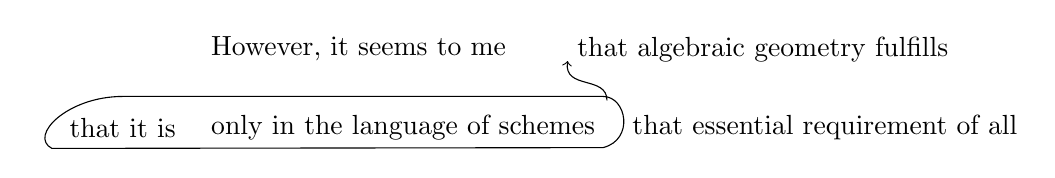
\begin{tikzpicture}[x=1cm,y=1cm]
\node[anchor=west] at (0,1) {However, it seems to me};
\node[anchor=west] at (4.65,1) {that algebraic geometry fulfills};
\node[anchor=west] at (-1.8,0) {\inserted{that it is}};
\node[anchor=west] at (0,0) {only in the language of schemes};
\node[anchor=west] at (5.35,0) {that essential requirement of all};
\draw (-1.9,-.26) .. controls (-2.2,-.1) and (-1.7,.4) .. (-1,.4) -- (5.1,.4) .. controls (5.4,.4) and (5.5,-.15) .. (5.1,-.25) -- (-1.9,-.26);
\draw[->] (5.15,.35) .. controls (5.15,.67) and (4.6,.48) .. (4.65,.85);
\end{tikzpicture}}
contemporary mathematics: to state its definitions and theorems in their natural abstract and formal setting in which they can be \deleted{considered} \inserted{developed} independently of geometric intuition. Moreover, it seems to me incorrect to assume that any geometric intuition is lost thereby: for example, the underlying variety in an algebraic scheme is rediscovered, and perhaps better understood through the concept of geometric points. As another example, the theory of schemes has made it possible, in a very intuitive way, to finally dispose of that famous embar\inserted{r}assment to

\mspage{33}
